\documentclass{beamer}
%
% Choose how your presentation looks.
%
% For more themes, color themes and font themes, see:
% http://deic.uab.es/~iblanes/beamer_gallery/index_by_theme.html
%
\mode<presentation>
{
  \usetheme{default}      % or try Darmstadt, Madrid, Warsaw, ...
  \usecolortheme{beaver} % or try albatross, beaver, crane, ...
  \usefonttheme{structuresmallcapsserif}  % or try serif, structurebold, ...
  \setbeamertemplate{navigation symbols}{}
  \setbeamertemplate{caption}[numbered]
} 

\usepackage[english]{babel}
\usepackage[utf8x]{inputenc}
\usepackage{multirow}
\usepackage{natbib}
\bibliographystyle{abbrvnat}
\usepackage[ruled]{algorithm2e}
\usepackage{booktabs}
\usepackage{subcaption}
\usepackage{xcolor} % http://www.ctan.org/tex-archive/macros/latex/contrib/xcolor
\usepackage{tikz}
\usetikzlibrary{fit,calc}
%define a marking command
\newcommand*{\tikzmk}[1]{\tikz[remember picture,overlay,] \node (#1) {};\ignorespaces}
%define a boxing command, argument = colour of box
\newcommand{\boxit}[1]{\tikz[remember picture,overlay]{\node[yshift=3pt,fill=#1,opacity=.25,fit={(A)($(B)+(.95\linewidth,.8\baselineskip)$)}] {};}\ignorespaces}
%define some colours according to algorithm parts (or any other method you like)
\colorlet{pink}{red!40}
\colorlet{blue}{cyan!60}

\newcommand{\R}{\mathbb{R}}
\newcommand{\N}{\mathbb{N}}
\newcommand{\E}{\mathbb{E}}
\DeclareMathOperator*{\argmax}{argmax}
\DeclareMathOperator*{\argmin}{argmin}
\newcommand{\norm}[1]{\left\lVert#1\right\rVert}

\title{Flat Clustering Algorithms for Big Data}
%references:
%https://tex.stackexchange.com/questions/280713/creating-author-blocks-in-beamer-using-authblk-package
%https://cn.sharelatex.com/learn/Beamer
\author{Yuanhang Ren \\ 201721220117 \\ \texttt{ryuanhang@gmail.com}}
\institute{School of Information and Software Engineering \\ University of Electronic Science and Technology of China}

\begin{document}

% make title page
\begin{frame}
  \titlepage
\end{frame}

% Uncomment these lines for an automatically generated outline.
% \begin{frame}{Outline}
%  \tableofcontents
% \end{frame}
\AtBeginSection[]
{
  \begin{frame}
    \frametitle{Table of Contents}
    \tableofcontents[currentsection] 
  \end{frame}
}
\AtBeginSubsection[]
{
	\begin{frame}
		\frametitle{Table of Contents}
		\tableofcontents[ 
		sectionstyle=show/hide,
		subsectionstyle=show/shaded/hide, 
		] 
	\end{frame}
}

\section{Introduction}

\begin{frame}{Clustering}

\begin{itemize}
  \item What is clustering?
%   reference:
%   https://stackoverflow.com/questions/144639/how-to-order-citations-by-appearance-using-bibtex
% 	https://tex.stackexchange.com/questions/103192/cite-author-and-number-index
% 	https://tex.stackexchange.com/questions/340056/cite-and-footnote-in-together-in-beamer
% 	https://tex.stackexchange.com/questions/315627/how-to-cite-a-reference-on-beamer-as-author-year/315632
  \item Flat clustering vs Hierarchical clustering
\end{itemize}

\begin{figure}
\centering
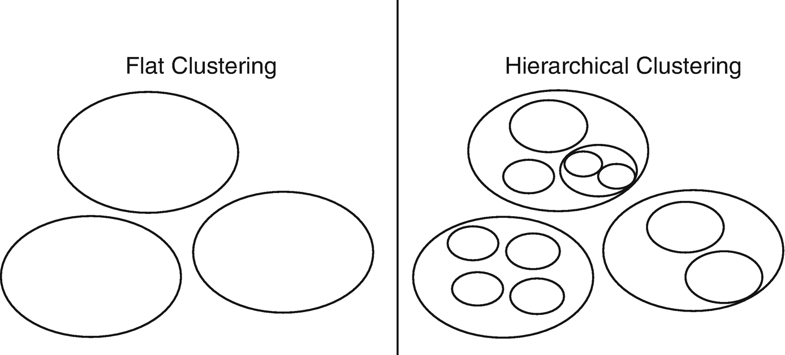
\includegraphics[scale=0.2]{clustering_types.png}
\end{figure}

\end{frame}

\begin{frame}{Research Problems}
Traditional clustering algorithms might be inefficient when datasets are huge and they are also not theoretically guaranteed.

Hence, we focus on clustering algorithms that are:
\begin{itemize}
	\item provably good
	\item efficient
\end{itemize}

We are going to design and analyze such algorithms on the \textit{$k$-means} and \textit{spectral clustering} problems. 

\end{frame}

\section{$k$-means}

\subsection{Backgrounds}

\begin{frame}{$k$-means problem}

\begin{itemize}
	\item It is well-known due to the Lloyd algorithm \citep{lloyd1982least} (a.k.a $k$-means algorithm)
	\item The $k$-means problem is NP-hard
\end{itemize}
\begin{definition}[$k$-means problem]
	Given $n$ data points $\mathcal{X} \subseteq \R^d$ and a set of $k$ points $C \subseteq \R^d$, where $d$ is the dimension of the data point. An objective function is defined as follows,
	\begin{equation}
		\phi_C(\mathcal{X}) = \sum_{x \in \mathcal{X}}d^2 (x,C)
	\end{equation}
	where $d(x,C) = \min\limits_{c \in C}\norm{x - c}$ is the distance of a point to a set. The $k$-means problem is to find the optimal $C$ such that the $\phi_C(\mathcal{X})$ is minimized given $\mathcal{X}$.
\end{definition}

\end{frame}

\begin{frame}{The Solution Quality}
	\begin{definition}[Solution Quality 1]
		Let $\alpha \geq 1$. A set $C$ of $k$ centers is an $\alpha$ approximation solution of $k$-means if
		\begin{equation}
		\phi_C(\mathcal{X}) \leq \alpha \phi_\text{OPT}(\mathcal{X})
		\end{equation}
		$\phi_\text{OPT}(\mathcal{X})$ is the minimal objective.
	\end{definition}
	\begin{definition}[Solution Quality 2]
		Let $\alpha \geq 1$ and $\beta > 0$. A set $C$ of $k$ centers is a $\beta$-bad $\alpha$-approximation solution of $k$-means if
		\begin{equation}
		\phi_C(\mathcal{X}) > (\alpha + \beta)\phi_\text{OPT}(\mathcal{X})
		\end{equation}
		Otherwise, $C$ is said to be a $\beta$-good $\alpha$-approximation.
	\end{definition}
\end{frame}

\subsection{Provably Good Algorithms}

\begin{frame}{$k$-means++}
	$k$-means++ \citep{arthur2007k} employs the \textit{$d^2$ weighting} to achieve a $O(\log k)$ guarantee.
	% ref: https://tex.stackexchange.com/questions/220589/how-to-scale-algorithm-to-fit-in-one-frame-and-centered-in-the-frame-at-same-tim
	
	\scalebox{0.8}{
		\begin{minipage}{0.7\linewidth}
			\begin{algorithm}[H]
				\caption{$k$-means++ seeding}
				\KwIn{dataset $\mathcal{X}$, number of centers $k$}
				\KwOut{$k$ centers $C$}
				$c_1 \gets $ Sample a point uniformly at random from $\mathcal{X}$ \\
				$C \gets \{c_1\}$ \\
				\For{$i = 2,3, \ldots k$}{
					\For{$x \in \mathcal{X}$}{
						% we can calculate a small set of p instead of whole p(x)
						$p(x) \gets \text{d}(x,C)^2/\sum_{x' \in \mathcal{X}} \text{d}(x',C)^2$
					}
					$x \gets$ Sample a point from $\mathcal{X}$ using $p(x)$ \\
					$C \gets C\cup\{x\}$
				}
				\textbf{return} $C$
			\end{algorithm}
		\end{minipage}
	}%
	\begin{minipage}{0.3\linewidth}
		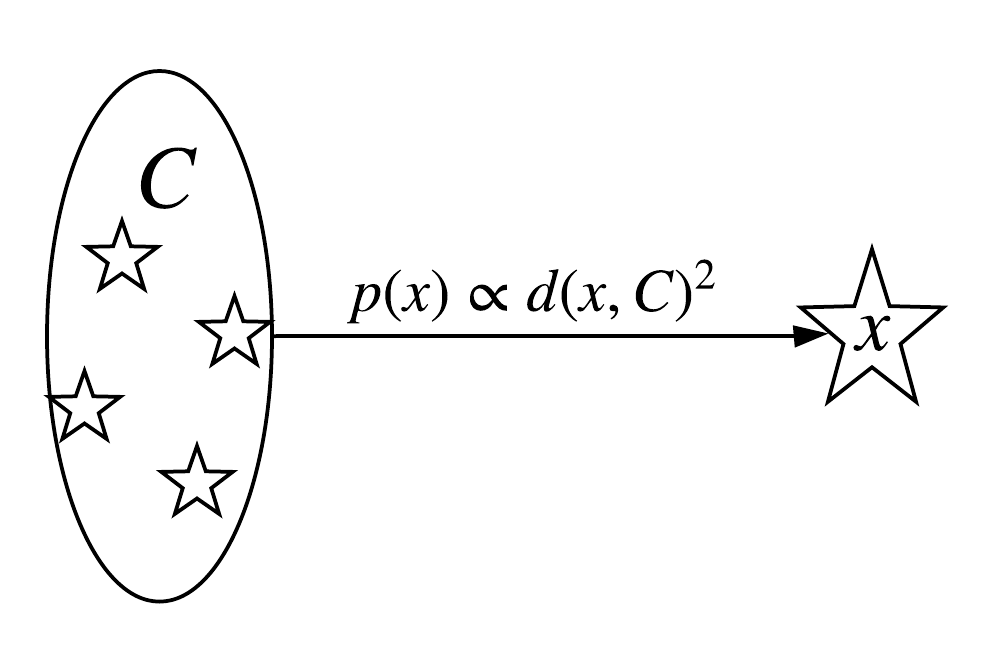
\includegraphics[scale=0.5]{kmeans++.png}
	\end{minipage}

\end{frame}

\begin{frame}{$k$-means\(\vert \vert\)}
	
	The $k$-means\(\vert \vert\) \citep{bahmani2012scalable} accelerates the $k$-means++
	
	\scalebox{0.7}{
		\begin{minipage}{0.88\linewidth}
			\begin{algorithm}[H]
				\caption{$k$-means\(\vert \vert\) seeding}
				\KwIn{dataset $\mathcal{X}$, oversampling factor $l$, number of centers $k$, number of rounds $t$}
				\KwOut{$k$ centers $C$}
				$S \gets$ Sample a point uniformly at random from $\mathcal{X}$\\
				\For{i = 1,2,...,t}{
					$C' \gets \emptyset$ \\
					\For{$x \in \mathcal{X}$}{
						Add $x$ to $C'$ with probability $\min(1,\frac{ld^2 (x,S)}{\phi(\mathcal{X},S)})$
					}
					$S \gets  S \cup C'$
				}
%				ref: https://tex.stackexchange.com/a/386274
				\tikzmk{A}
				For $s \in S$, set $w_s$ to be the number of points in $\mathcal{X}$ closer to $s$ than any other point in $S$ \\
				$C \gets$ Let $w_s$ be the weights of $s$ and run an $\alpha$ approximation algorithm on the weighted $S$ \\ 
				\tikzmk{B}
				\boxit{blue}
				\textbf{return} $C$
			\end{algorithm}
		\end{minipage}
	}%
	\begin{minipage}{0.3\linewidth}
		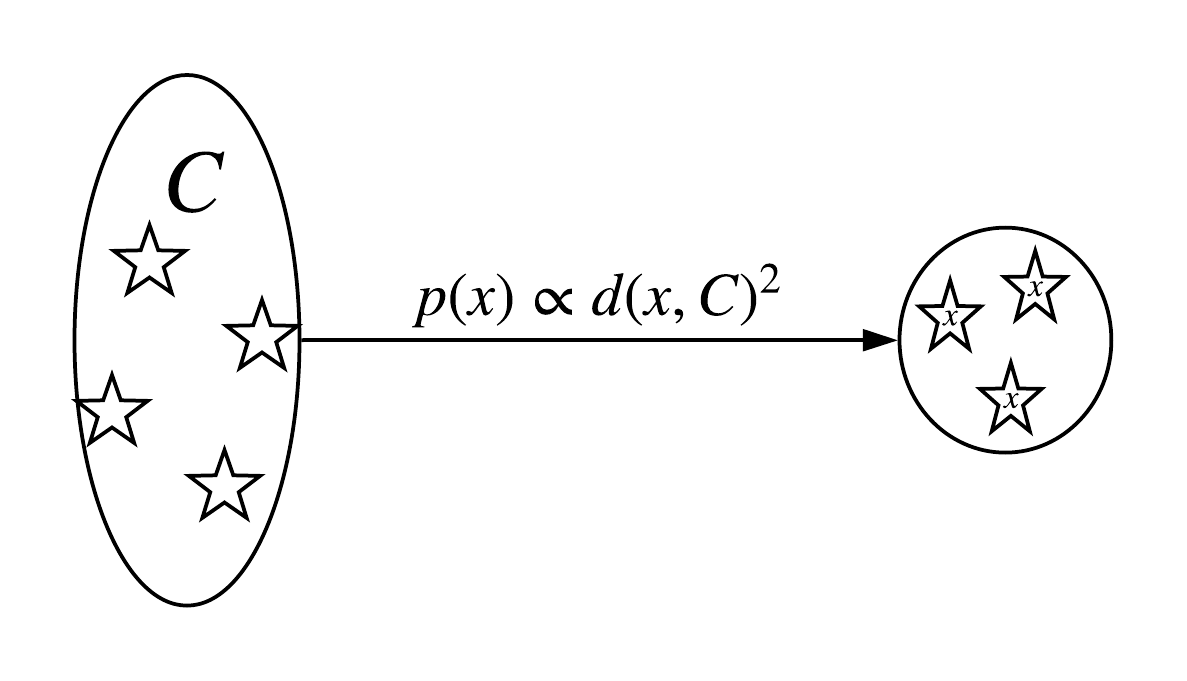
\includegraphics[scale=0.4]{kmeans||.png}
	\end{minipage}
	
\end{frame}

\begin{frame}{The First Contribution}
	The classic $k$-­means++ algorithm has been extended to weighted $k$-­means problem and proofs on the clustering quality are given.
	
\end{frame}

\begin{frame}{The Weighted $k$-means Problem \& Algorithm}
	\begin{definition}[weighted $k$-means problem]
		\footnotesize
		Given $n$ data points $\mathcal{X} \in \R^d$ and associated weights $w$. Find a set of $k$ points $C \subseteq \R^d$, such that the following objective function is minimized.
		\begin{equation}
		\psi_C(\mathcal{X})=\sum_{x_i \in \mathcal{X}}w_i d^2(x_i,C)
		\end{equation}
	\end{definition}
	\vspace*{-0.5cm}
	\begin{center}
		\scalebox{0.7}{
			\begin{algorithm}[H]
				\caption{weighted $k$-means++ seeding}
				\KwIn{dataset $\mathcal{X}$, data weights $w$, number of centers $k$}
				\KwOut{$k$ centers $C$}
				$c_1 \gets $ Sample a point from $\mathcal{X}$ with probability $\frac{w_x}{\sum_{i \in \mathcal{X}} w_i}$ \\
				$C \gets \{c_1\}$ \\
				\For{$i = 2,3, \ldots k$}{
					\For{$x \in \mathcal{X}$}{
						% we can calculate a small set of p instead of whole p(x)
						$p(x) \gets w_x\text{d}(x,C)^2/\sum_{x' \in \mathcal{X}} w_x'\text{d}(x',C)^2$
					}
					$x \gets$ Sample a point from $\mathcal{X}$ with $p(x)$ \\
					$C \gets C\cup\{x\}$
				}
				\textbf{return} $C$
			\end{algorithm}
		}
	\end{center}
	
\end{frame}

\begin{frame}{Guarantee of Weighted $k$-means++}
	\begin{theorem}[quality of weighted $k$-means++]
		Given data points $\mathcal{X}$ and associated weights $w$. Let $C$ be the results returned by the weighted $k$-means++. We have
		\begin{equation}
			\E[\psi_C(\mathcal{X})] \leq 8(\ln k + 2) \psi_\text{OPT}(\mathcal{X})
		\end{equation}
	\end{theorem}
	The big picture of the proof:
	\begin{itemize}
		\item Consider the quality of the uniform sampling
		\item Consider the quality of the $d^2$ weighting
		\item Show relationships between intermediate results by induction
	\end{itemize}
\end{frame}

\begin{frame}{Picture of The Proof}
	\begin{lemma}[quality of uniform sampling]
		Given an arbitrary optimal cluster $A$. Denote $Z$ be the chosen point with probability $\frac{w_z}{\sum_{i \in A} w_i}$. Then, $\E[\psi_Z(A)] = 2 \psi_{\text{OPT}}(A)$
	\end{lemma}
	\begin{lemma}[quality of $d^2$ weighting]
		Let $C$ be the arbitrary intermediate results, $1 \leq |C| \leq k-1$. Denote $A$ be an arbitrary optimal cluster and let $Z \in A$ be the chosen point using $d^2$ weighting given $C$. Then, we have $\E[\psi_{C'}(A)|C,Z \in A] \leq 8 \psi_{\text{OPT}}(A)$, where $C' = C \cup \{Z\}$.
	\end{lemma}
\end{frame}

\begin{frame}{Picture of The Proof}
%	\scalebox{0.8}{text}
	\begin{lemma}[relationships of intermediate results]
		\footnotesize
		Let $C$ be the arbitrary intermediate results, $1 \leq |C| \leq k-1$. Choose $u>0$ "uncovered" optimal clusters, and let $\mathcal{X}_u$ denote the set of points in these clusters. Also let $\mathcal{X}_c = \mathcal{X} - \mathcal{X}_u$. Suppose we add $0 \leq t \leq u$ points with $d^2$ weighting given $C$. Denote $C'$ as the resulting points. Then, 
		\begin{equation}
		\E[\psi_{C'}(\mathcal{X})|C] \leq [\psi_C(\mathcal{X}_c)+8\psi_{\text{OPT}}(\mathcal{X}_u)](1+H_t)+\frac{u-t}{u}\psi_C(\mathcal{X}_u)
		\end{equation}
		where $H_t = 1+\frac{1}{2}+...+\frac{1}{t}$ is the harmonic sum.
	\end{lemma}
	\begin{figure}
		\centering
		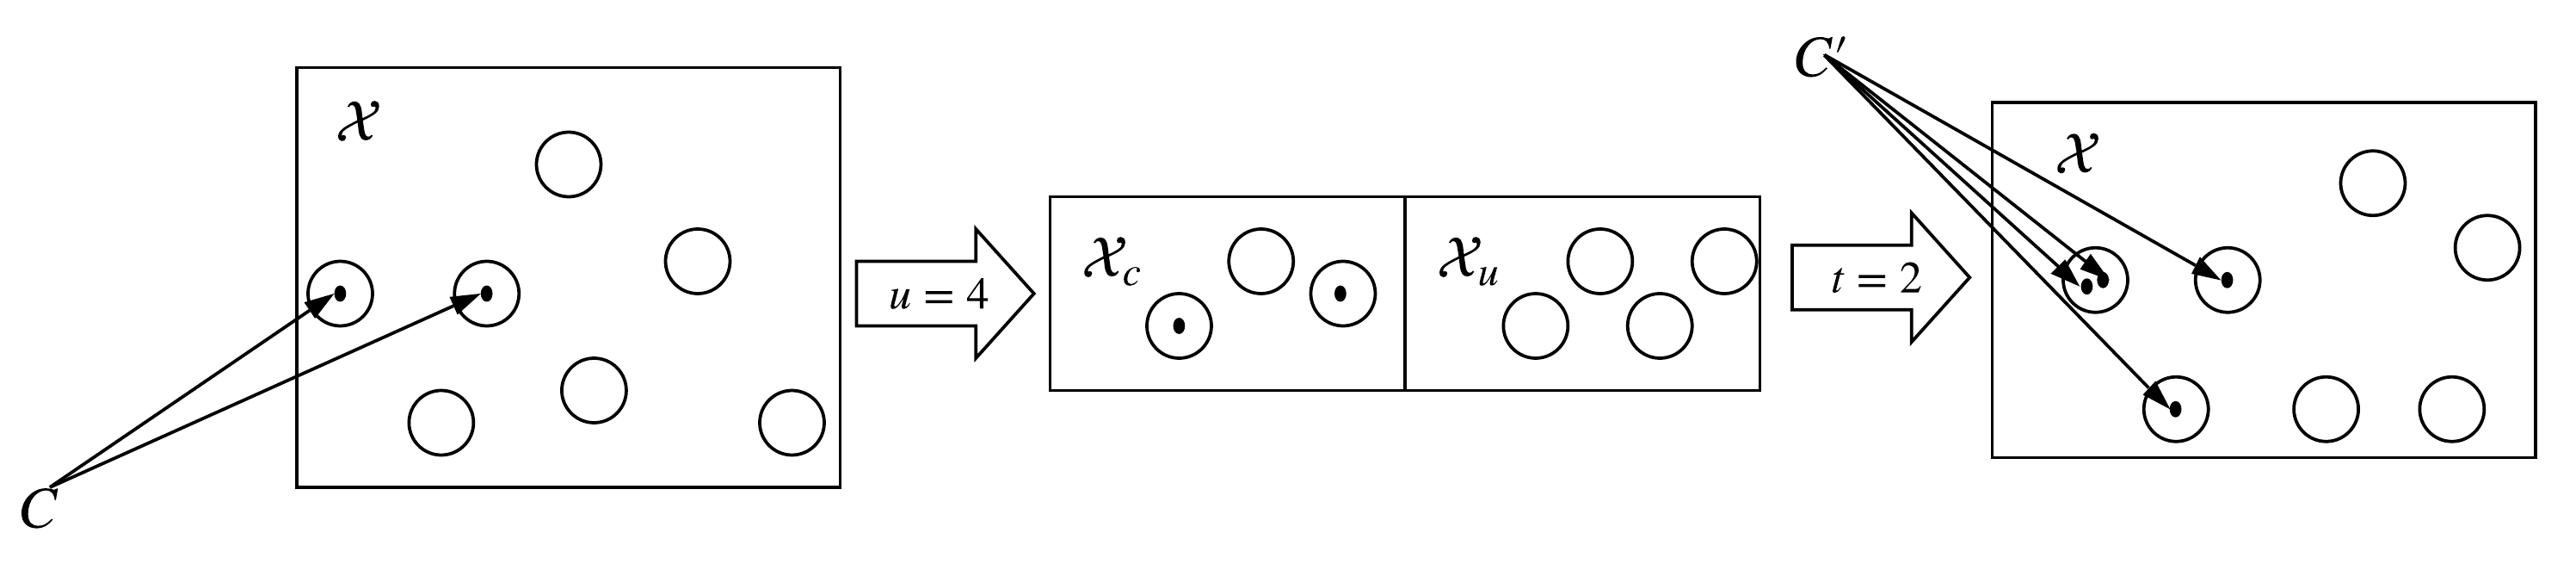
\includegraphics[scale=0.4]{lemma_relationships.png}
	\end{figure}
\end{frame}

\subsection{Efficient Algorithms}


\begin{frame}{Clustering Based on Uniform Sampling}
%	\begin{itemize}
%		\item reduce data size
%		\item uniform sampling works well
%	\end{itemize}
	\vspace*{-0.2cm}
	\begin{center}
		\scalebox{0.7}{\begin{algorithm}[H]
				\label{alg:clustering based on uni w/o}
				\caption{clustering based on uniform sampling}
				\KwIn{dataset $\mathcal{X}$, number of clusters $k$, number of points to sample $s$, clustering algorithm $\mathcal{A}_c$}
				\KwOut{$k$ centers $C$}
				$S \gets$ Sample $s$ points uniformly without replacement \\
				$C \gets$ Solve the $k$-means problem on $S$ with $\mathcal{A}_c$ \\
				\textbf{return} $k$ centers $C$
			\end{algorithm}}
		\scalebox{0.7}{
			\vbox{
				\begin{theorem}[quality of Algorithm \ref{alg:clustering based on uni w/o}]
					Let $0 < \delta <1/2$, $\alpha \geq 1$, $\beta >0$ be approximation parameters. Let C be the set of centers returned by Algorithm \ref{alg:clustering based on uni w/o} and $\mathcal{A}_c$ is an $\alpha$ approximation algorithm. Suppose we sample $s$ points uniformly without replacement such that,
					\begin{equation*}
					s \geq \ln(\frac{1}{\delta})(1+\frac{1}{n})/(\frac{\beta^2 m^2}{2\Delta^2 \alpha^2}+\frac{\ln(1/\delta)}{n})
					\end{equation*}
					we have
					\begin{equation*}
					\phi_C(\mathcal{X}) \leq \textcolor{red}{4(\alpha + \beta)} \phi_\text{OPT}(\mathcal{X})
					\end{equation*}
					with probability at least $1-2\delta$, where $\Delta = \max\limits_{i,j}\norm{v_i - v_j}^2$ is the squared diameter of the data, $m = \phi_\text{OPT}(\mathcal{X})/n$ is the average of the optimal objective.
				\end{theorem}
			}
		}
	\end{center}
\end{frame}

\begin{frame}{The Second Contribution}
	\begin{itemize}
		\item A sharper bound for the uniform sampling algorithm is proved, and a further proof indicate that this algorithm runs in polylogarithmic time given mild assumptions on datasets.
		\item A novel algorithm called Double-K-M$\text{C}^2$ is proposed to approximate weights.
		\item MATLAB implementations of uniform sampling, K-M$\text{C}^2$, Double-K-M$\text{C}^2$, and their corresponding kernel versions are given. Experiments are carried out to verify the efficiency and effectiveness of these algorithms.
	\end{itemize}
\end{frame}

\begin{frame}{A Sharper Bound}
	\vspace*{-0.7cm}
	\begin{center}
		\scalebox{0.7}{
			\vbox{
				\begin{theorem}[a sharper bound of uniform sampling]
					Let $0 < \delta <1/2$, $\alpha \geq 1$, $\beta >0$ be approximation parameters. Let C be the set of centers returned by Algorithm \ref{alg:clustering based on uni w/o} and $\mathcal{A}_c$ is an $\alpha$ approximation algorithm. Suppose we sample $s$ points uniformly without replacement such that,
					\begin{equation*}
					s \geq \ln(\frac{1}{\delta})(1+\frac{1}{n})/(\frac{\beta^2 m^2}{2\Delta^2 \alpha^2}+\frac{\ln(1/\delta)}{n})
					\end{equation*}
					we have
					\begin{equation*}
					\phi_C(\mathcal{X}) \leq \textcolor{red}{(\alpha + \beta)} \phi_\text{OPT}(\mathcal{X})
					\end{equation*}
					with probability at least $1-2\delta$, where $\Delta = \max\limits_{i,j}\norm{v_i - v_j}^2$ is the squared diameter of the data, $m = \phi_\text{OPT}(\mathcal{X})/n$ is the average of the optimal objective.
				\end{theorem}
			}
		}
	\end{center}
	\vspace*{-0.3cm}
	The big picture of the proof:
	\begin{enumerate}
		\scriptsize
		\item Show that $C$ will be a \textit{good} solution for $S$.
		\item Suppose $C$ is a \textit{bad} solution for $\mathcal{X}$, it will probably be a \textit{bad} solution for $S$.
		\item According to 1 and 2, $C$ will be a \textit{good} solution for $\mathcal{X}$
	\end{enumerate}
\end{frame}

\begin{frame}{A Poly-Log Time Algorithm}
	Assume that a dataset is sampled i.i.d. according to a
	probability distribution $F$
	%todo which distributions satisfy these two assumptions?
	\begin{itemize}
		\item $F$ has finite variance and exponential tails, \textit{i.e.} $\exists c,t$ such that $P[\text{d}(x,\mu(F))>a]\leq ce^{-at}$, where $\mu(F)$ is the mean of $F$.
		\item $F$'s minimal and maximal density on a hypersphere with non zero probability mass is bounded by a constant.
	\end{itemize}
	\begin{theorem}[efficiency of uniform sampling]
		\small
		Let $0 < \delta <1/2$, $\alpha \geq 1$, $\beta >0$ be approximation parameters. Assume (A1) and (A2) hold, and let $C$ be the set of centers returned by Algorithm \ref{alg:clustering based on uni w/o}, we have the following 
		\begin{equation*}
		\phi_C(\mathcal{X}) \leq (\alpha + \beta)\phi_\text{OPT}(\mathcal{X})
		\end{equation*}
		with probability at least $1-2\delta$ if we sample $O(\ln(\frac{1}{\delta})\frac{\alpha^2}{\beta^2}k^2\log^4 n)$ points
	\end{theorem}
\end{frame}

\subsection{Experiments}

\begin{frame}{Baseline Algorithms}
	\begin{itemize}
		\footnotesize
		\item Since the uniform sampling algorithm is efficient and provably good, we design experiments to verify this.
		\item Baselines are K-M$\text{C}^2$ \citep{bachem2016approximate} and Double-K-M$\text{C}^2$ sampling.
		\item As computing weights in $k$-means\(\vert \vert\) is time-consuming, we propose a novel algorithm called \textit{Double-K-M$\text{C}^2$ sampling} to approximate weights.
	\end{itemize}
	\begin{center}
		\scalebox{0.7}{\begin{algorithm}[H]
				\caption{Double-K-M$\text{C}^2$ sampling}
				\KwIn{dataset $\mathcal{X}$, \# of points to sample $s$, chain length $u$}
				\KwOut{$k$ centers $C$}
				$S_1 \gets $ Sample $s$ points from $V$ via K-M$\text{C}^2$ \\
				$V' \gets $ Remove $S_1$ from $V$ \\
				$S_2 \gets $ Sample $s$ points from $V'$ via K-M$\text{C}^2$ \\
				For point $s_i \in S_1$, let $w_i$ be the number of points in $S_2$ closer to $s_i$ than to any other points in $S_1$ \\
				Let $w_i + 1$ be the weight of $s_i$ \\
				$C \gets$ Solve the weighted $k$-means problem on $S_1$ with an $\alpha$ approximation algorithm \\
				\textbf{return} $k$ centers $C$
			\end{algorithm}}
	\end{center}
	
\end{frame}

\begin{frame}{Traditional Clustering}
	\begin{center}
		\scalebox{0.7}{
			\vbox{
				\begin{table}[H]
					\caption{data size $n$, number of clusters $k$, dimension $d$}
					\begin{tabular}{cccc}
						\toprule
						datasets & $n$ & $k$ & $d$ \\
						\midrule
						a2 & 5250 & 35 & 2 \\
						a3 & 7500 & 50 & 2 \\
						b2-random-10 & 10000 & 100 & 2 \\
						b2-random-15 & 15000 & 100 & 2 \\
						b2-random-20 & 20000 & 100 & 2 \\
						\midrule
						KDD & 145751 & 200 & 74 \\
						RNA & 488565 & 200 & 8 \\
						Poker Hand & 1000000 & 200 & 10 \\
						\bottomrule
					\end{tabular}
				\end{table}
			}	
		}
	\end{center}
	\begin{itemize}
		\scriptsize
		% todo Lloyd algorithm iterations?
		\item chain length: $u=200$
		\item sampling size: $1.5 \log^2 n$ and $0.7 \log^4 n$ for Double-K-M$\text{C}^2$ and uniform sampling
		\item $\alpha$ approximation algorithm: (weighted) $k$-means++ with Lloyd
		\item evaluation metrics: number of distance evaluations and $k$-means objective
		\item algorithms are run 40 times repeatedly with different initial random seeds
	\end{itemize}
\end{frame}

\begin{frame}{Results}
	\begin{minipage}{0.4\linewidth}
		\scriptsize
		\begin{enumerate}
			\item The time cost of uniform sampling is about
			10 times higher than that of K-M$\text{C}^2$ and it increases slowly with
			respect to the data size. The $k$-means objective of uniform sampling is
			roughly 60\% of the objective of K-M$\text{C}^2$.
			\item Double-K-M$\text{C}^2$ achieves a better clustering quality compared
			with K-M$\text{C}^2$ and a lower time cost compared with uniform sampling.
			\item Double-K-M$\text{C}^2$ could be the first choice if you prefer a good clustering quality with reasonable time costs. For the best quality, uniform sampling is recommended.
		\end{enumerate}
	\end{minipage}
	\scalebox{0.55}{
		\begin{minipage}{1.0\linewidth}
			\begin{figure}[H]
				\centering
				\begin{subfigure}{0.493\columnwidth}
					\centering
					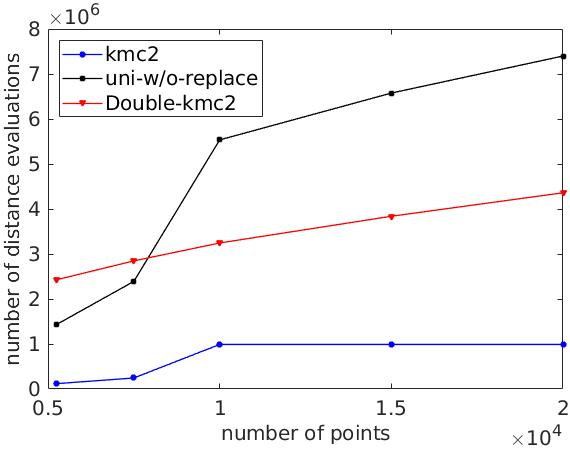
\includegraphics[width=\linewidth]{syn-running-time.jpg}
					\caption{\small{the number of distance evaluations on synthetic data}}
					\label{}
				\end{subfigure}
				\hfill
				\begin{subfigure}{0.493\columnwidth}  
					\centering 
					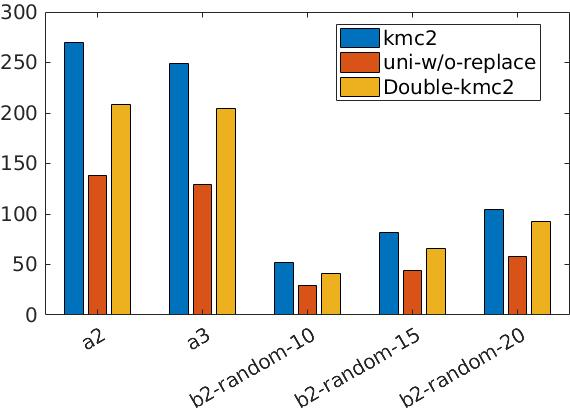
\includegraphics[width=\linewidth]{syn-sum-squared-distances.jpg}
					\caption{\small{$k$-means objective on synthetic data}}
					\label{}
				\end{subfigure}
				\vskip\baselineskip
				\begin{subfigure}{0.493\columnwidth}   
					\centering 
					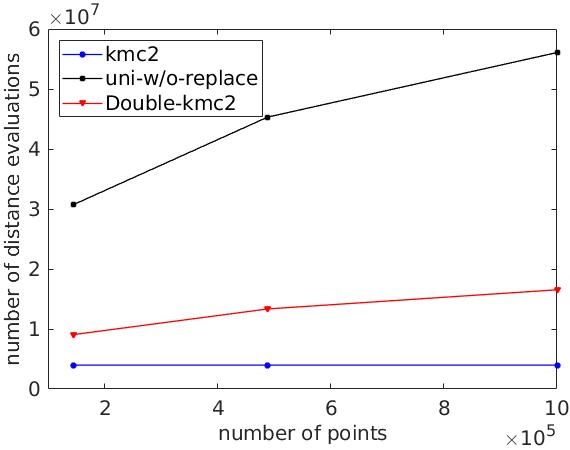
\includegraphics[width=\linewidth]{real-running-time.jpg}
					\caption{\small{the number of distance evaluations on real data}}    
					\label{}
				\end{subfigure}
				\hfill
				\begin{subfigure}{0.493\columnwidth}
					\centering 
					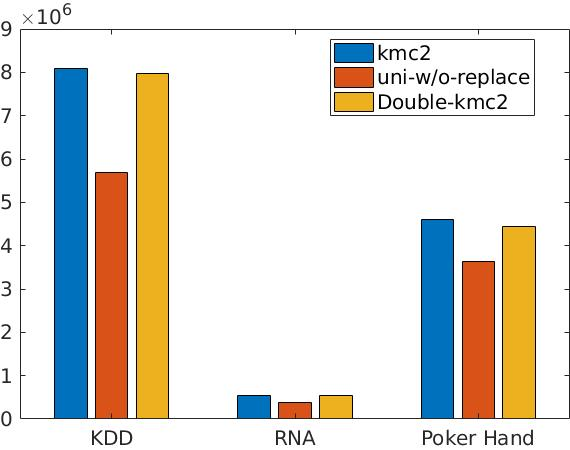
\includegraphics[width=\linewidth]{real-sum-squared-distances.jpg}
					\caption{\small{$k$-means objective on real data}}    
					\label{}
				\end{subfigure}
				\caption{$k$-means objective and time cost versus the number of points}
				\label{fig:running time & sum of distances}
			\end{figure}
		\end{minipage}
%		\vbox{
%			
%		}
	}
	
\end{frame}

\begin{frame}{Image Segmentation}
	\begin{center}
		\scalebox{0.7}{
			\vbox{
				\begin{table}[H]
					\caption{data size $n$, number of clusters $k$}
					\begin{tabular}{ccc}
						\toprule
						datasets & $n$ & $k$ \\
						\midrule
						baby & 900(30 * 30) & 5 \\
						kitten & 3600(60 * 60) & 5 \\
						bear & 14400(120 * 120) & 5 \\
						\bottomrule
					\end{tabular}
				\end{table}
			}
		}
	\end{center}
	\begin{itemize}
		\scriptsize
		\item The kernel versions of uniform sampling, Double-K-M$\text{C}^2$, and K-M$\text{C}^2$.
		\item Construct an affinity matrix $A$ via the approach in \citet{stella2003multiclass} and find the nearest positive definite matrix $K$ as the kernel.
		\item chain length: $u=200$
		\item sampling size: $0.25\log^2 n$ and $0.4\log^4 n$ for Double-K-M$\text{C}^2$ and uniform sampling
		\item $\alpha$ approximation algorithm: (weighted) kernel $k$-means++ with kernel Lloyd
		\item evaluation metric: number of distance evaluations and kernel $k$-means objective
		\item algorithms are run 30 times repeatedly with different initial random seeds
	\end{itemize}
\end{frame}

\begin{frame}{Results}
	\begin{minipage}{0.4\linewidth}
		\scriptsize
		\begin{enumerate}
			\item The kernel uniform sampling has the best clustering quality while the growth of the time cost is not too rapid. 
			\item The kernel Double-K-M$\text{C}^2$ has a similar clustering quality with much lower time cost compared with the kernel uniform sampling. 
			\item Thus, we recommend using kernel Double-K-M$\text{C}^2$ if the quality is your major concern. For a more efficient result, the kernel K-M$\text{C}^2$ is a better choice.
		\end{enumerate}
	\end{minipage}
	\scalebox{0.55}{
		\begin{minipage}{1.0\linewidth}
			\begin{figure}[H]
				\centering
				\begin{subfigure}{0.493\columnwidth}   
					\centering 
					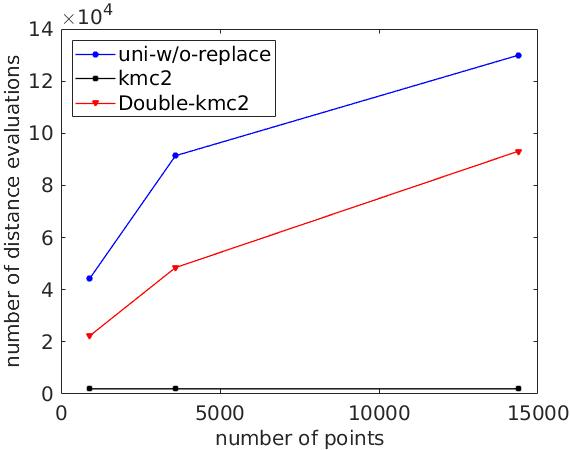
\includegraphics[width=\linewidth]{image-running-time.jpg}
					\caption{the number of distance evaluations on image data}
				\end{subfigure}
				%	    \begin{minipage}{0.494\columnwidth}
				%	        \centering
				%	        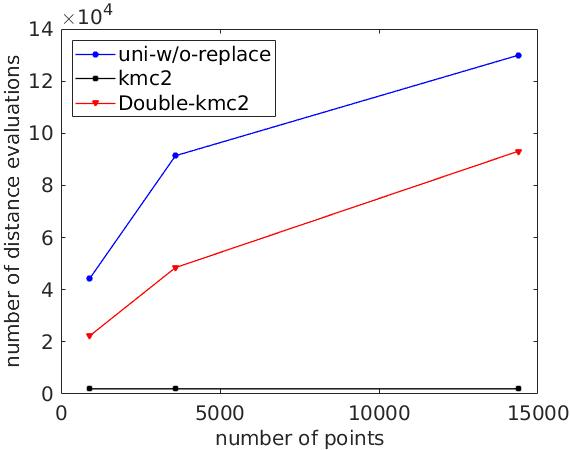
\includegraphics[width=\linewidth]{image-running-time.jpg}
				%	    \end{minipage}
				%	    \hfill
				\begin{subfigure}{0.493\columnwidth}   
					\centering 
					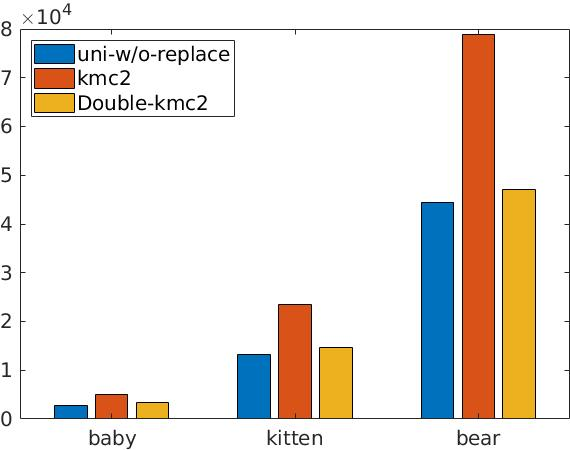
\includegraphics[width=\linewidth]{image-obj.jpg}
					\caption{kernel $k$-means objective on image data}
				\end{subfigure}
				
				%	    \begin{minipage}{0.494\columnwidth}
				%	        \centering
				%	        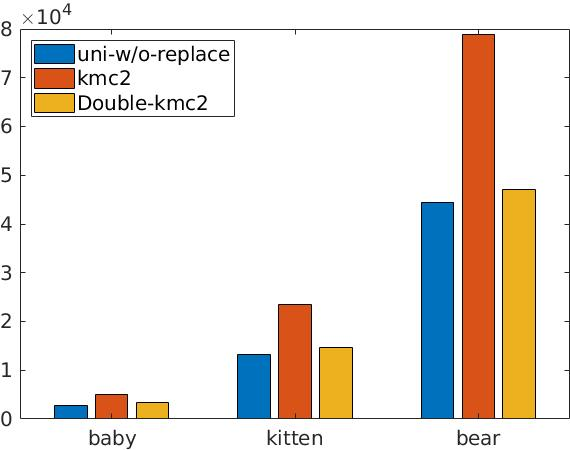
\includegraphics[width=\linewidth]{image-obj.jpg}
				%	    \end{minipage}
				
%				\caption{(Left) . (Right) }
				\caption{kernel $k$-means objective and time cost versus the number of points}
				\label{fig: image running time & ncut}
			\end{figure}
		\end{minipage}
		%		\vbox{
		%			
		%		}
	}
	
\end{frame}

\section{Spectral Clustering}

\subsection{Backgrounds}

\begin{frame}{Spectral Clustering Problem}
	\begin{itemize}
		\item The problem is introduced from the graph theory.
		\item This problem is also NP-hard.
	\end{itemize}
	\begin{definition}[Normalized Cut]
		Denote $v_i$ as the node $i$ and $C_j$ as the cluster $j$. Find a partition matrix $F_{ij} = \begin{cases} 1 & {v_i \in C_j} \\ 0 & {otherwise}
		\end{cases}$, such that the following objective is minimized,
		\begin{equation}
			\min\limits_{F} \operatorname{Tr}(\frac{F^T L F}{F^T D F})
		\end{equation}
		where $L = D-A$, $A$ is the affinity matrix of the graph, and $D$ is the degree matrix of $A$.
	\end{definition}
\end{frame}

\subsection{Provably Good and Efficient Algorithms}

\begin{frame}{Transform into Traditional Clustering}
	\footnotesize{
		\begin{definition}[weighted kernel $k$-means problem]
			Given $n$ data points $\mathcal{X} \subseteq \R^d$, associated weights $w$, and a mapping function $\varphi(.)$. Find a set $C$ of size $k$ such that the following objective is minimized,
			\begin{equation}
			\Psi_C(\mathcal{X}) = \sum_{i=1}^k \sum_{x_j \in \pi_i}w_j \norm{\varphi(x_j)-C_i}^2
			\end{equation}
			where $\pi_i$ is the $i$th cluster, $\cup_{i=1}^k \pi_i = \mathcal{X}$, $C_i = \frac{\sum_{x_j \in \pi_i}w_j \varphi(x_j)}{\sum_{j \in \pi_i}w_j}$.
		\end{definition}
	}
	\footnotesize{
		\begin{lemma}[relationships between two clusterings]
			Let $W$ and $K$ be the weight and kernel matrix of the weighted kernel $k$-means. Choose $W=D$ and $K=D^{-1}AD^{-1}$, where $D$ and $A$ are the degree and affinity matrix of the spectral clustering. Then, we have
			\begin{equation}
			\Psi_C(\mathcal{X})=\operatorname{Tr}(D^{-1/2}AD^{-1/2})-k+Ncut
			\end{equation}
		\end{lemma}
	}
	
\end{frame}

\begin{frame}{The Uniform Sampling Algorithm}
	\vspace*{-0.25cm}
	\begin{center}
		\scalebox{0.67}{\begin{algorithm}[H]
				\SetNoFillComment
				\caption{uniform sampling and weighted kernel $k$-means based spectral clustering \citep{Mohan:2017:BNA:3172077.3172235}}\label{alg: uniform_wkk}
				\KwIn{dataset $\mathcal{X}$, number of clusters $k$, sample size $s$, affinity matrix $A$, degree matrix $D$}
				\KwOut{$k$ partitions of $\mathcal{X}$}
				$S \gets$ Sample $s$ numbers uniformly from $1,2,...,n$ without replacement\\
				$W \gets D,K \gets D^{-1}AD^{-1}$\\
				$W_s \gets W(S,S), K_s \gets K(S,S)$\\
				$\pi' \gets$ Run an $\alpha$ approximation algorithm on $S$ given $W_s$ and $K_s$\\
				\tcc{diffuse}
				\For{$i = 1,...,n$}{
					\For{$c = 1,...,k$}{
						\begin{equation*}
						d(a_i,m_c) \gets K_{i i}-\frac{2 \sum_{a_{j} \in \pi'_{c}} w_{j} K_{i j}}{\sum_{a_{j} \in \pi'_{c}} w_{j}}+\frac{\sum_{a_{j}, a_{l} \in \pi'_{c}} w_{j} w_{l} K_{j l}}{\left(\sum_{a_{j} \in \pi'_{c}} w_{j}\right)^{2}}
						\end{equation*}\\
					}
					$j \gets \argmin\limits_{c = 1,2,...,k} d(a_i,m_c)$\\
					$Y_{ij} \gets 1$
				}
				\textbf{return} $Y$
			\end{algorithm}}
		\end{center}
\end{frame}

\begin{frame}{The Third Contribution}
	\begin{itemize}
		\item A sharper bound for the uniform sampling and weighted kernel $k$-means based spectral clustering algorithm has been proved.
		\item We give MATLAB implementations of this algorithm and use experiments to validate the efficiency and the quality of it.
	\end{itemize}
\end{frame}

\begin{frame}{A Sharper Bound}
	\begin{theorem}[a sharper bound of Algorithm \ref{alg: uniform_wkk}]
		Let $0 < \delta <1/2$, $\alpha \geq 1$, and $\beta >0$ be approximation parameters. Suppose we sample $s$ points in Algorithm \ref{alg: uniform_wkk} such that,
		\begin{equation}
		s \geq \ln(\frac{1}{\delta})(1+\frac{1}{n})/(\frac{\beta^2 m^2}{2\Delta^2 \alpha^2}+\frac{\ln(1/\delta)}{n})
		\end{equation}
		we have
		\begin{equation}
		Ncut \leq \textcolor{red}{(\alpha + \beta)} Ncut^* + (\alpha + \beta -1)c
		\end{equation}
		with probability at least $1-2\delta$, where $\Delta = \max\limits_{i,j}\norm{\varphi(x_i) - \varphi(x_j)}^2$ is the squared diameter of the data in the mapped space, $m = \Psi_\text{OPT}(\mathcal{X})/n$ is the average of the optimal objective, $c$ is a constant irrelevant to partitions, $Ncut^*$ is the optimal $Ncut$.
	\end{theorem}
\end{frame}

\subsection{Experiments}

\begin{frame}{Traditional Clustering}
	\begin{center}
		\scalebox{0.7}{
			\vbox{
				\begin{table}[H]
					\caption{data size $n$, number of clusters $k$, dimension $d$}
					\label{tab:datasets_spectral_clustering}
					\begin{tabular}{ccccc}
						\toprule
						datasets & name & $n$ & $d$ & $k$ \\
						\midrule
						$D_1$ & segment &2310 & 19 & 7 \\
						$D_2$ & MnistData-05 &3495 &784 & 10 \\
						$D_3$ & MnistData-10 &6996 & 784 & 10 \\
						$D_4$ & isolet5 &7797 & 617 & 26 \\
						$D_5$ & USPS &9298 & 256 & 10 \\
						$D_6$ & letter-recognition &20000 & 16 & 26 \\
						\bottomrule
					\end{tabular}
				\end{table}
			}	
		}
	\end{center}
	\begin{itemize}
		\scriptsize
		\item Experiments will be performed to verify the efficiency and the effectiveness of uniform sampling
		\item algorithms: weighted kernel $k$-means(uniform sampling vs no-sampling)
		\item anchor based graph construction method
		\item sampling size: 20\% of data points
		\item $\alpha$ approximation algorithm: weighted kernel $k$-means++
		\item evaluation metrics: time(s) and Ncut
	\end{itemize}
\end{frame}

\begin{frame}{Results}
	\begin{minipage}{0.4\linewidth}
		\scriptsize
		\begin{enumerate}
			\item The sampling version is about 20$\sim$50 times faster than the no-sampling one while Ncut is not larger than the no-sampling version by 25\%
			\item Hence, the uniform sampling method is a good choice for its amazing efficiency and reasonable clustering quality.
		\end{enumerate}
	\end{minipage}
	\scalebox{0.57}{
		\begin{minipage}{1.0\linewidth}
			\begin{figure}[H]
				\begin{subfigure}{.49\linewidth}
					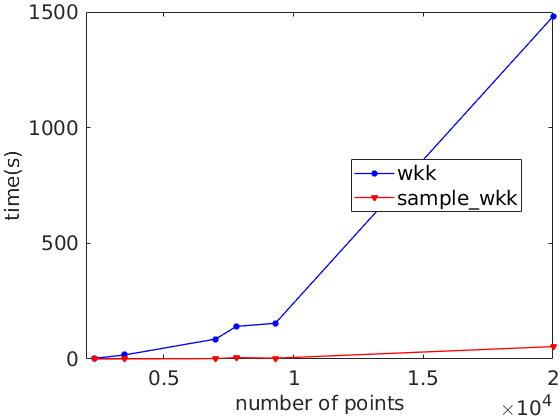
\includegraphics[width=\linewidth]{sp-running_time.jpg}
					\caption{time costs(s)}
				\end{subfigure}
				\begin{subfigure}{.49\linewidth}
					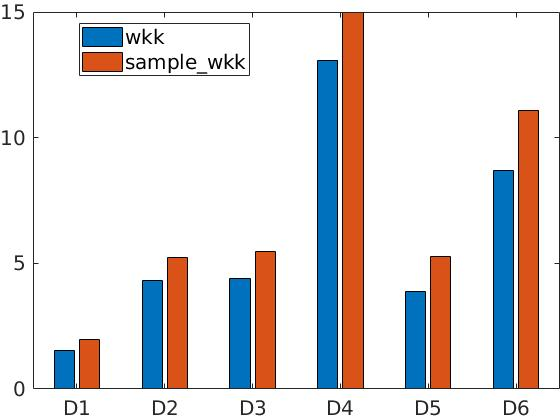
\includegraphics[width=\linewidth]{sp-Ncuts.jpg}
					\caption{Ncut}
				\end{subfigure}
				\caption{results of spectral clustering}
				\label{fig: sp-experiments}
			\end{figure}
		\end{minipage}
		%		\vbox{
		%			
		%		}
	}
	
	
	
\end{frame}

\section{Summary of Contributions}

\begin{frame}{Summary}
	\begin{enumerate}
		\small
		\item (Theoretical) The classic $k$-­means++ algorithm has been extended to weighted $k$-­means problem and proofs on the clustering quality are given.
		\item (Theoretical) A sharper bound for the uniform sampling algorithm on $k$-means is proved, and a further proof indicates that this algorithm runs in polylogarithmic time given mild assumptions on datasets.
		\item (Theoretical) A sharper bound for the spectral clustering is proved.
		\item (Empirical) We give MATLAB implementations of uniform sampling, K-M$\text{C}^2$, Double-K-M$\text{C}^2$, and their corresponding kernel versions on $k$-means. Experiments validate the efficiency and effectiveness of these algorithms.
		\item (Empirical) We give MATLAB implementations of the weighted kernel $k$-means based spectral clustering algorithm and its corresponding sampling versions. Experiments are used to justify these algorithms on the efficiency and solution quality.
	\end{enumerate}
\end{frame}

% reference:
% https://tex.stackexchange.com/questions/86101/beamer-creating-a-slide-with-short-centered-prominent-text
\begin{frame}[plain,c]
\begin{center}
\Huge Questions?
\end{center}
\end{frame}

\begin{frame}{References}
	\scriptsize
    \bibliographystyle{unsrt}
    \bibliography{bibfile}
\end{frame}

\end{document}
